\section{Introduction}

Flooding is one of the most significant natural disasters in the United States (US) affecting both the loss of life and property. 
In 2017 and 2019, river and flash flooding combined represented the leading cause of death among all natural disasters and in 2018 they were only second to deaths from heat wave\cite{national_weather_service_2020,national_weather_service_2019,national_weather_service_2018}. 
More than an average of 104 deaths per year are attributed to flood events from the 10 year period ending in 2019 \cite{us_department_of_commerce_2020}. 
Within that 10 year window, the most common activity victims were partaking in is driving year after year when compared to walking/hiking, at home, boating, fell in, working, and other \cite{us_department_of_commerce_2020}.
With respect to property damages, river and flash flooding have contributed to 60.7, 1.6, and 3.7 billion non-inflation adjusted US dollars in the annual periods of 2017 to 2019, respectively \cite{national_weather_service_2020,national_weather_service_2019,national_weather_service_2018}. 
The large spike in damages for 2017 can be attributed to the Hurricane Harvey event that primarily affected Texas in August. 
Unencouragingly, the trends related to flood damages and fatalities have been steadily increasing over recent decades. \cite{mallakpour2015changing,downton2005reanalysis,kunkel1999temporal,pielke2000precipitation,corringham2019effect}. 
Some are expecting that the hydrologic cycle will intensify which will lead to more extreme precipitation in some areas along with a greater risk of flooding \cite{tabari2020climate,milly2002increasing,wing2018estimates}. 
Increasing trends in frequency and risk are not uniform across spatial regions with work by \citeA{slater2016recent} indicating that trends are increasing across the US Midwest/Great Lakes region while decreasing in coastal Southeast, Southwest and California.


Operational flood forecasting systems are primary tools in developing accurate forecasts for public awareness prior to life or property damaging events occur. 
One of these operational systems is the Advanced Hydrologic Prediction System (AHPS) maintained by National Oceanic Atmospheric Administration (NOAA) National Weather Service (NWS) with approximately 3,781 forecast points across the US at typically short forecast horizons of 24 or 72 hours\cite{mcenery2005noaa}.
AHPS provides forecasting services in the form of ensemble streamflows at 3,781 forecast points illustrated in \ref{fig:all_ahps_points} and flood inundation maps (FIM) at 188 of those forecast points shown in \ref{fig:fim_ahps_points}.
AHPS implements a series of advances including model calibration techniques \cite{zhang2003hydrologic,hogue2003multi,duan2003global,gupta2003advances,parada2003multi}, distributed modeling approaches \cite{reed2004overall,koren2004hydrology,duan2002results}, ensemble forecasting \cite{day1985extended,seo2000simulation,mullusky2002simplified,herr2002simplified}, enhanced data analysis procedures \cite{mcenery2005noaa}, flood-forecasting inundation maps \cite{cajina2002fldview}, hydraulic routing models \cite{fread1973technique,cajina2002fldview}, and multisensor precipitation techniques \cite{breidenbach1999accounting,kondragunta2001outlier,seo2002real,bonnin1996noaa}.
Despite the AHPS advances in operational flood forecasting its significant limitations are the lack of spatial coverageand short forecast time horizons.
Approximately, there is only one forecast point every 1,455 km of river and one forecast point with FIM every 29,261 km.


Additional work is required to fill-in the gaps that the AHPS leaves in terms of spatial and temporal coverage.
To broaden the forecasting domain, the Office of Water Prediction (OWP) at the National Water Center (NWC) in Tuscaloosa, Alabama commissioned the utilization of the National Water Model (NWM) which is an instance of the Weather Research and Forecast Hydrologic Model (WRF-Hydro) \cite{gochis2018wrf,cosgrove2019evolution}. 
The NWM forecasts river discharges at more than 2.7 million forecast points at a variety of time horizons including some medium (10 day) and long (30 day) range forecast horizons.
The NWM enhances the spatial and temporal domain of the current AHPS capabilities at the 13 River Forecast Centers (RFC) in areas known as "hydro-blind" and is not meant to be a replacement. 
It's simply an additional model to be used in the forecasting and early warning decision making.


The National Hydrography Dataset Plus (NHDPlus) version 2.1 is the basis for the hydrofabric in the NWM due to its comprehensive use with the hydrologic communities' stakeholders \cite{mckay2012nhdplus}. 
The term hydrofabric is used within the NWM jargon to describe the collection of geospatial datasets required for modeling including but not limited to stream networks, catchments, channel properties, and elevation data. 
The routing methods used within the NWM for its stream network is Muskingam-Cunge (MC) routing \cite{bedient2008hydrology,ponce1994variable,gochis2018wrf}.






\begin{figure}
\centering
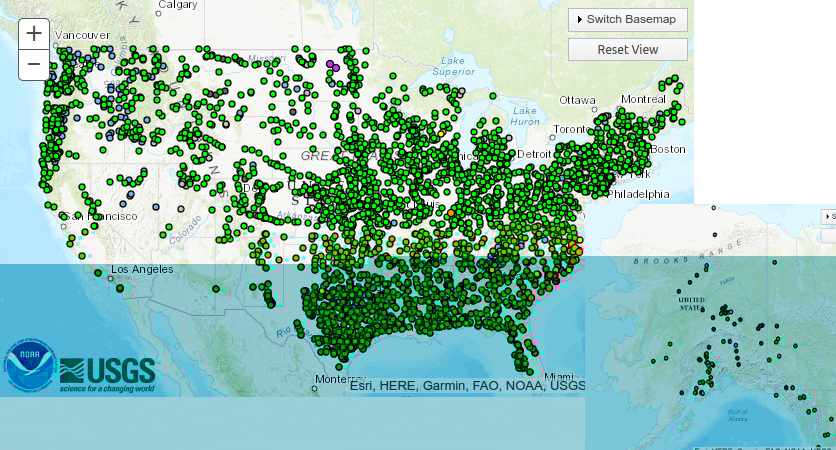
\includegraphics[scale=2.0]{figs/ahps_all_forecast_points.jpg}
\label{fig:all_ahps_points}
\caption{All 3,781 forecast points in United States' Advanced Hydrologic Prediction System for lower 48 states and Alaska. No forecast points in Hawaii or territories. From: water.weather.gov/ahps}
\end{figure}


\begin{figure}
\centering
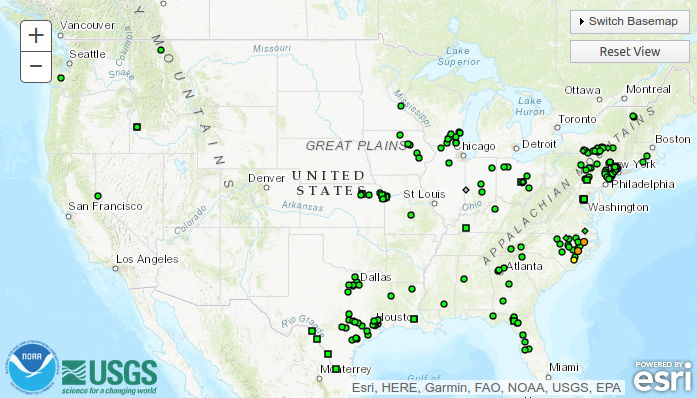
\includegraphics[scale=2.0]{figs/ahps_fim_forecast_points_conus.jpg}
\label{fig:fim_ahps_points}
\caption{All 188 forecast points in United States' Advanced Hydrologic Prediction System with flood inundation mapping capabilities. One forecast point near Juneau, Alaska not shown. No forecast points in Hawaii or remaining territories. From: water.weather.gov/ahps}
\end{figure}
